\chapter{Evolutionary Game Theory}
\label{evolutionary-game-theory}

\setlength{\epigraphwidth}{.9\textwidth}
\epigraph{We repeat most emphatically that our theory is thoroughly static. A dynamic theory would unquestionably be more complete and preferable.\\ --\citet[44-45]{von-neumann-morgenstern1944}\\ \hspace{12pt}

We shall now take up the ``mass-action'' interpretation of equilibrium points...It is unnecessary to assume that the participants have full knowledge of the total structure of the game, or the ability and inclination to go through any complex reasoning process.\\
--\citet[21]{nash1950}
%There are many situations, however, in which an individual is, in effect, competing not against an individual opponent but against the population as a whole.\\ --\citet[23]{maynard-smith1982}
}

Game theory is a branch of applied mathematics originally developed by \cite{von-neumann-morgenstern1944} that models human decision-making when the actions, outcomes, and preferences of multiple agents are intertwined. This differs from decision theory, where a single agent is faced with a choice to bring about his or her most preferred outcome. Rather, a game arises when the choices made by each player crucially depend on those made by others. It is this interdependence that distinguishes game theory and makes it such a useful tool in understanding social interactions, from the routes we choose to drive to work to the way we use words to mean things.

While 



The rest of this chapter provides an outline of the crucial concepts for our application of evolutionary game theory to language change. First, we offer a general overview of the dimensions along which games vary. We focus on two simple games, and develop intuitions about expected behavior. Second, we define a set of solution concepts that can be applied to predict behavior in the two simple games. We discuss the limitations of solutions concepts for predicting behavior. Third, we supply game dynamics and examine the trajectory of the population under those game dynamics for the two simple games. We then we define signaling games as a natural model of communication and present the simplest case. Finally, we present a generalized means of describing the dynamics of arbitrarily complex signaling games.


Taking up one aspect of this first example, we will assume that the vast majority of people would prefer to avoid car accidents. When driving a car, this is straightforwardly achievable by always being on the opposite side of the road of the next oncoming vehicle. We can think about this from the perspective of two drivers approaching each other. Each driver has the choice of driving on the left or the right. Both parties would prefer to coordinate on driving on whichever side. The side of the road that best achieves the outcome of not crashing is irrelevant, but it depends on how both parties drive. If both parties choose to drive on the right, from their own perspective, then they will avoid each other. Likewise if they choose to drive on the left.

The solutions to this interaction are readily apparent, everyone should choose one side of the road or the other. Provided that both drivers choose the same side, then neither has an incentive to switch. This fundamental insight into behavior in games is what defines a \emph{Nash equilibrium}: the action of all agents is optimal given the choices of all other agents. Yet, grounding this solution in rationalistic terms requires a little more effort. First, it requires that all agents are \emph{rational}, acting to maximize their own benefit. This is implicit in our example above, most humans prefer to avoid being injured. Second, it requires that players have \emph{common knowledge} of the game structure, including the actions available to all players, the outcomes of different combinations, and know that they all know these things, and so forth. At least for this game it follows naturally from the number of sides of the road there are, and the ability to reason about collisions, but it is not always so straightforward. Finally, it requires that agents have \emph{equilibrium knowledge}, that they are able to accurately anticipate the actions of other players.  This last requirement may seem readily apparent, at least for the example of driving, but it deserves further comment. 

Depending on the country, we know that everyone will drive on one side of the road. In fact, there are laws and legal repercussion for not doing so. Yet, if we abstract away from our everyday experience in this particular case, the problem becomes clearer. For example, imagine that you are asked to choose between two options, that another person has been asked to choose between the same two options, that both of you have received the same instructions, and that you will both succeed if you choose the same option. These starker terms may seem to border on the absurd, but they bring the problem into relief. Their absurdity lies in the fact that it does not do to reason about \emph{this} option or \emph{that} option, because there is nothing to distinguish the two. There is no \emph{thisness} or \emph{thatness} to motivate one choice or the other. That is, there is no rule of the road that simply states "Drive on the right". Instead, we are faced with the problem of deciding the undecidable, as Aristotle, a bit sarcastically put it in his \emph{On the Heavens}:
%Buridanian 

\begin{quotation}
%men who, though exceedingly hungry and thirsty, and both equally, yet being equidistant from food and drink, is therefore bound to stay where he is-even so
[A] man, being just as hungry as thirsty, and placed in between food and drink, must necessarily remain where he is and starve to death.
\end{quotation}

We are particularly good at looking for reasons why one option is preferable, or more likely to be chosen than another. For example, if we were to enrich our description above to a choice between an option \emph{A} or an option \emph{B}, an intuitive rationale would be to choose \emph{A}. The reason for doing so being that \emph{A} comes first in the alphabet, and that both people might expect each other to know this. There is some intuitive \emph{thisness} about option \emph{A} that we can leverage on the assumption that it will be readily apparent to others as well.  \citet[57]{schelling:1960} called these partial escapes from the dilemma of equilibrium knowledge \emph{focal points} ``for each person�s expectation of what the other expects him to expect to be expected to do." In the pre-cellular age, Schelling posed the following scenario: ``Tomorrow you have to meet a stranger in NYC. Where and when do you meet them?" The intuitive meeting place of Schelling's day was Grand Sentral station at noon. The rationale for both choices is that they are prominent in their respective geographical and temporal landscapes. Experimental results demonstrate that people are generally quite  good at grounding their coordination via reasoning about these kinds of focal points \citep{mehta-etal1994,mehta-etal1994b,bardsley-etal2010}. 


But, even with our ability to reason about what we might expect others to expect us to expect them to expect us to do, we still cannot perfectly anticipate what others will do. That is, focal points are useful heuristics, but they are never foolproof: not everyone would choose option \emph{A} or grand central station at noon. In fact, it would not be foolish for example to suggest meeting at Times Square at noon. The problem of justifying equilibrium in general still remains. Nash himself was well aware of this problem, which was in part what prompted his consideration of a ``mass-action'' interpretation of equilibria.\footnote{The main motivation was understanding \emph{mixed Nash equilibria}, which involve some probability distribution over actions. \cite{nash1950,nash:1950,nash:1951} proved that such an equilibrium is guaranteed to exist. What it means for an individual to adopt the corresponding \emph{mixed strategy} is not unproblematic. For a discussion of these problems see \cite{aumann1985}, and for the population approach see \cite{rosenthal1979}.} In short, this change in perspective moves from focusing on a single agent to a population of agents that need not have either common knowledge or equilibrium knowledge.  This perspective was naturally taken up in applications of game theory to biology, where loosening some of the equilibrium requirements was both reasonable and necessary \citep{maynard-smith1982}. This move also came with the reinterpretation of the game-theoretic machinery: actions were not choices to be made by the individual, but genetically pre-determined responses; the utility derived from a particular outcome was not a numerical representation of preferences, but a measure of Darwinian \emph{reproductive fitness}. 

This turn towards the biological allowed for further developments towards the explicitly dynamic theories that \cite{von-neumann-morgenstern1944} envisioned.  Drawing on the mechanics of population genetics, \cite{taylor-jonker:1978} offered the first \emph{evolutionary game dynamics}, christened the \emph{replicator dynamics} by  \cite{eigen-schuster1979}, which explicitly defined how a population changes over time due to biological reproduction.  This new approach allowed for insights into not just whether a population would remain at some equilibrium state if it started there, but also if the population would reach that equilibrium state in the first place. While successively detailed refinements of Nash equilibria were proposed with more and more unrealistic assumptions, evolutionary game theory offered a means of understanding equilibrium behavior under much simpler assumptions. 

Despite its biological roots, however, work in evolutionary game theory has discovered profound connections with the rationalistic approach to equilibrium behavior. That is, the equilibrium predictions of the rationalistic approach often correspond to the effect of natural selection captured by evolutionary game dynamics. Perhaps more surprisingly, some of these game dynamics can be derived not just from the mechanics of biological reproduction, but from particular kinds of decision making or behavior. For example, the replicator dynamics defined by \cite{taylor-jonker:1978} can also be derived from particular forms of imitation \citep{schlag1998,bjornerstedt-weibull1996} and learning \citep{borgers-sarin1997}. The fact that such  diverse foundations yield the same dynamics is both surprising and compelling. More importantly, these commonalities show that if we interpret \emph{evolution} in this broader sense that includes both biological and social change, then evolutionary game theory can serve as a powerful tool.

The rest of this chapter provides an outline of the crucial concepts for our application of evolutionary game theory to language change. First, we offer a general overview of the dimensions along which games vary. We focus on two simple games, and develop intuitions about expected behavior. Second, we define a set of solution concepts that can be applied to predict behavior in the two simple games. We discuss the limitations of solutions concepts for predicting behavior. Third, we supply game dynamics and examine the trajectory of the population under those game dynamics for the two simple games. We then we define signaling games as a natural model of communication and present the simplest case. Finally, we present a generalized means of describing the dynamics of arbitrarily complex signaling games.


\section{Games}
\label{Games}

There are several major dimensions along which games can vary.\footnote{See \cite{dixit-skeath2004} for a gentle introduction to game theory, \cite{tadelis2013} for a thorough but balanced introduction, and \cite{osborne-rubinstein1994} and \cite{fudenberg-tirole1991} for more advanced mathematical treatments.} Here we focus on several dimensions that are relevant for the case of communication and thus language change.  The first dimension we will consider is the order which players make their decisions. If all players make a decision at the same time, then the game is a \emph{simultaneous} game. If players make their decisions in a particular order, then the game is a \emph{sequential} game. Communication is sequential insofar as we separate out the transmission and interpretation of a signal. Thus, we will be concerned with sequential games.

The second dimension along which games vary is whether or not players have private information that affects others' payoffs. If players do have private information then the game is one \emph{incomplete information}, otherwise it is one of \emph{complete information}. Intuitively, this is the crucial aspect of communication. Speakers have some private information  that hearers do not. We cannot read minds, thus we have to communicate. This asymmetry of information is crucially tied to the third dimension along which games vary. Namely, if the set of actions available to the different players differs or if the payoff from the same action differs, then the game is considered \emph{asymmetric}. If the actions are identical for all players and if the outcome of actions are independent of who takes them then the game is \emph{symmetric}. There are clearly two distinct roles in the act of communication, thus we will be concerned with asymmetric sequential games of incomplete information.

In this section we introduce to simple simultaneous games of complete information.  We develop the intuitions required for the application of equilibrium concepts and dynamic analysis before moving on to the more complicated asymmetric sequential games of incomplete information known as \emph{signaling games} that will be used in subsequent analysis. 

%
%The final dimension along which games vary is whether the players have the same or similar preferences over outcomes. 
%
%The space of possibilities is fairly large, but there are indeed several broad distinctions between classes of games.



%If they do, then we call the game one of \emph{common interests}. If they do not, then we call the game one of \emph{conflicting interests}. A special case of conflicting interests is where players have perfectly opposing interests, a gain for one player is an equal and opposite loss for the other. These kinds of games are \emph{constant} or \emph{zero-sum games}.

%We vary whether the games are constant-sum or not, and hence games of common or conflicting interests as well as symmetric versus asymmetric.

%Interestingly, there are some logical relationships between these dimensions. For example, a game of incomplete information is necessarily asymmetric. Likewise, a constant-sum game is also asymmetric. 

The first simple example we consider is parallel to the case of choosing which side of the road to drive on, and is often referred to as a \emph{coordination game}. There are two players who we will refer to as \emph{Row} and \emph{Column}, for reasons that will become clear later on. Each player has a choice between two options, \emph{A} and \emph{B}. We we will refer to these options as \emph{pure strategies}.\footnote{This is in contrast to \emph{mixed} strategies, which specifiy a probability distribution over pure sender strategies, $\sigma = p_1 s_1 + ... + p_k s_k$, where $\sum_i p_i = 1$.}  That is, the set of pure strategies available to \emph{Row} is $S_R = \{A, B \}$, and the set of actions available to \emph{Column} is $S_C = \{A, B \}$. The set of all combinations of \emph{Row} and \emph{Column} strategies constitute the \emph{strategy profiles} of the game. That is, for each $s_i \in S_R$ and $s_j \in S_C$, the tuple $\langle s_i, s_j \rangle$ constitutes a strategy profile. 

Now, we can capture the intuition that both players prefer to avoid crashing by defining utility functions over outcomes for both players. \emph{Row}'s utility function is a function from strategy profiles to real numbers $U_R : \langle s_i, s_j \rangle \rightarrow \mathbb{R}$. Likewise \emph{Column}'s utility function is a function from strategy profiles to real numbers $U_C : \langle s_j, s_i \rangle \rightarrow \mathbb{R}$. In fact, we can drop the subscripts entirely, if we define the two utility functions in the following way.

\begin{equation}
U(s_i, s_j) = U_{R}(s_i, s_j) =  U_{C}(s_j, s_i) =
\left\{
	\begin{array}{ll}
		1  & \mbox{if } s_i = s_j \\
		0 & \mbox{else}
	\end{array}
\right.
\end{equation}
Note that utilities are only important insofar as they represent an ordinal ranking over outcomes. In other words, there is nothing particularly special about $0$ and $1$ as opposed to say $3.277$ and $110$ other than the fact that in both cases the first is less than the second. However, there is something important about the fact that $U(A, A) = U(B, B)$. This simply reflects the fact that either rule of the road is equally useful for avoiding collisions.

With these utility functions defined, we can present the game in a slightly more compact \emph{normal form} as in Table \ref{CG}. The strategies for \emph{Row} and \emph{Column} are listed to the left and above respectively, hence the names. By convention, for each cell of Table \ref{CG}, the payoff for \emph{Row} is listed first, followed by the payoff for \emph{Column}. The reason why coordination games are symmetric is that both $U_R$ and $U_C$ define symmetric matrices. Intuitively, we could rotate Table \ref{CG} around its diagonal and nothing would change;  the payoffs for one player are the transpose of the other. In fact, we could represent the payoffs in this symmetric game as a matrix that captures this symmetry.

\begin{table}\centering
\begin{tabular}{lll}
\hline\noalign{\smallskip}
 & A & B \\
\noalign{\smallskip}\hline\noalign{\smallskip}
A & $1, 1$ & $0, 0$ \\
B & $0, 0$ & $1, 1$ \\
\noalign{\smallskip}\hline
\end{tabular}
\caption{Coordination Game}
\label{CG}
\end{table}


\begin{equation}
U(s_i, s_j) = 
 \begin{pmatrix}
 1 & 0\\
 0 & 1\\
 \end{pmatrix}
\end{equation}


With these definitions in place, we return to the reasoning above. Namely, both players want to coordinate on playing either $A$ or $B$. If one player chooses $A$, then the other should as well. If one player chooses $B$, then the other should as well. But, there is no guarantee that the other player will choose $A$ or $B$. Again, simply knowing that both would be good outcomes does not guarantee that both players will choose one or the other.

We can modify the game in a simple but substantial way by altering the payoff structure. That is, imagine the case where the utility functions of the sender and receiver are defined as the following.

\begin{equation}
 U_{R}(s_i, s_j) =
\left\{
	\begin{array}{ll}
		1  & \mbox{if } s_i \neq s_j \\
		0 & \mbox{else}
	\end{array}
\right.
\end{equation}

\begin{equation}
 U_{C}(s_j, s_i) =
\left\{
	\begin{array}{ll}
		1  & \mbox{if } s_i = s_j \\
		0 & \mbox{else}
	\end{array}
\right.
\end{equation}
That is, the payoffs of \emph{Row} are diametrically opposed to that of \emph{Column}. This game, called \emph{matching pennies} has the following simple rules. Both players choose between heads $H$ or tails $T$. One player wins if the coins match, and the other player wins if the coins do not match. The resulting game is summarized in Table \ref{MP}. Matching pennies is a constant-sum asymmetric game, the components of every cell in Table \ref{MP} sum to a constant. Except in the trivial case where all outcomes yield the same utility for both players, constant-sum games are asymmetric. That is, we cannot represent the payoffs as a single value without losing crucial information.  


\begin{table}\centering
\begin{tabular}{lll}
\hline\noalign{\smallskip}
 & H & T \\
\noalign{\smallskip}\hline\noalign{\smallskip}
H & $0, 1$ & $1, 0$ \\
T & $1, 0$ & $0, 1$ \\
\noalign{\smallskip}\hline
\end{tabular}
\caption{Matching Pennies}
\label{MP}
\end{table}
 Unlike the coordination game, players want to anti-coordinate with each other.  That is, if \emph{Row} plays $H$, then \emph{Column} would prefer to play $H$, but if \emph{Column} plays $H$ then \emph{Row} would prefer to play $T$. This poses another interesting problem. If both players have opposing interests, how should they act? It is clearly not feasible to pick one strategy or the other, as this would leave either player open to exploitation by the other. It would seem then that the best both players can do is to flip a coin and play whichever side comes up.

Before turning to defining equilibria, we need to note one last aspect of utility. As a case in point, let us assume that when playing matching pennies as \emph{Row}, we know that our opponent has a certain probability of playing $H$, and thus a certain probability of playing $T$. Let $p$ be the probability that our opponent plays $H$. Given that we are never certain of which strategy our opponent will play, we want to know the \emph{expected utility} of choosing one strategy or another. With slight abuse of notation, this is just the following.\footnote{This is just the expected value of a random variable. To take a simple example, imagine if we flipped a fair coin, counting heads as a $1$ and tails as a $0$, then the expected value of the coin flip would be $\frac{1}{2}$}

\begin{equation}
	E[U_R(H)] = pU_R(H,H) + (1-p)U_R(H,T) = (1-p)
\end{equation}
Expected utility is crucial in determining behavior in cases where there is uncertainty due to probabilistic behavior.

\section{Equilibria}

A game by itself does not constitute a model in the technical sense. It is a mathematical structure that describes the players preferences and strategies, but it does not predict their behavior. To do so it must be supplemented with a \emph{solution concept} that predicts the conditions under which particular outcomes will obtain. Here we define two related solution concepts, note how they apply to the simple games we defined above, and note their limitations for predicting behavior.

\subsection{Nash Equilbria}

Perhaps the most widely used solution concept is that of a \emph{Nash equilibrium}, which specifies when players have an incentive to unilaterally deviate from a given strategy profile. We provide a definition and apply the concept to our simple games.

For a given strategy profile where $s_i$ is the strategy of a particular player, let $s_{-i}$ be the set of strategies for all other players. We have the following definition.

\begin{definition}
 A strategy profile $\langle s_i^*, s_{-i}^*\rangle$ is a \emph{Nash equilibrium}
if and only if:
  \begin{itemize}
   \item $\forall i$, $\forall s_i \in S_i$, such that $s_i \neq s_i^*$, $E[U(s_i^*,s_{-i}^*)] \geq
E[U(s_i,s_{-i}^*)]$
  \end{itemize}
\end{definition}


%\begin{definition}
% A strategy profile $\langle s^*, r^*\rangle$ is a \emph{Nash equilibrium}
%if and only if:
%  \begin{itemize}
%   \item For all $s \in S$, such that $s \neq s^*$, $E[U_S(s^*,r^*)] \geq
%E[U_S(s,r^*)]$
%  \item For all $r \in R$, such that $r \neq r^*$, $E[U_R(s^*,r^*)] \geq
%E[U_S(s^*,r)]$
%  \end{itemize}
%\end{definition}

This simply states that no players can do better by individually changing his or her strategy from the equilibrium profile.  No one has an incentive to change, so everyone keeps doing what they are doing, hence the term equilibrium.  That is, every player's current strategy is a \emph{best response} to everyone else's. Note that this best response need not be unique to constitute an equilibrium. This follows from the fact that the inequalities in the definition are not strict. We can, however, impose uniqueness in these best responses by requiring that the inequalities in the definition be strict. A \emph{strict Nash equilibrium} results, meaning that players can only ever do worse if they unilaterally deviate from the equilibrium. 


%Strict Nash equilibria are thus a proper subset of Nash equilibria. 

%Since we are interested not just in the behavior of two individuals, but rather the aggregate behavior of a population, we want a broader notion of equilibrium. In particular, we might ask whether a given population is susceptible to change.

%The two conditions simply state that neither the sender nor the receiver can do better by individually changing his or her strategy from the equilibrium profile.  The sender's strategy is his \emph{best response} to the receiver's strategy, and the receiver's strategy is likewise her best response to the sender's strategy. Note that these best responses need not be unique to consitute an equilibrium. This follows from the fact that the inequalities in the definiton are not strict. We can, however, impose uniqueness in these best responses by requiring that the inequalities in the definition be strict. A \emph{strict Nash equilibrium} results, meaning that players can only ever do worse if they unilaterally deviate from the equilibrium. Strict Nash equilibria are thus a proper subset of Nash equilibria.

We can now apply this solution concept to the games we described above. First, we look at the coordination game. We already noted that coordinating on one strategy or the other seems to be an intuitive solution. The conditions for $\langle A, A \rangle$ and $\langle B, B \rangle$ to be Nash equilibrium are the following.

\begin{equation}
		E[U(A, A)] \geq E[U(B, A)]
\end{equation}

\begin{equation}
		E[U(B, B)] \geq E[U(A, B)]
\end{equation}
In fact, looking at the payoffs in Table \ref{CG}, both of these outcomes meet the definition of a strict Nash equilibrium. Both players can only do \emph{worse} by deviating from the equilibrium.

There is one last kind of equilibrium to consider. Imagine that both players choose $A$ with probability $p$ and $B$ with probability $(1-p)$. The expected utility for both pure strategies are the following.

\begin{equation}
	E[U(A)] = pU(A,A) + (1-p)U(A,B) = p
\end{equation}	

\begin{equation}
	E[U(B)] = pU(B,A) + (1-p)U(B,B) = (1 - p)
\end{equation}	
Note that these are equal to each other when $p=\frac{1}{2}$. Now suppose that an agent plays a mixed strategy $\sigma$ that strikes this balance by playing each strategy half of the time. We can show that this mixed strategy is a Nash equilibrium by comparing how another mixed strategy would fare against it. First, note that the expected utility of $\sigma$ against itself is $\frac{1}{2}$.

\begin{equation}
	\begin{split}
		E[U(\sigma, \sigma)] &= \frac{1}{2} \cdot \frac{1}{2}U(A,A) + \frac{1}{2} \cdot \frac{1}{2}U(A,B) + \frac{1}{2} \cdot \frac{1}{2}U(B,A) + \frac{1}{2} \cdot \frac{1}{2}U(B,B) \\
		&= \frac{1}{2}
	\end{split}
\end{equation}
Second, consider the expected utility of any alternate strategy $\sigma'$ that plays $A$ with probability $p$ and $B$ with probability $(1-p)$. Note that this includes the pure strategies as extremes, $A$ where $p=1$ and $B$ where $p=0$.

\begin{equation}
	\begin{split}
		E[U(\sigma', \sigma)] &= \frac{1}{2} \cdot pU(A,A)  + \frac{1}{2} \cdot pU(A,B) + \frac{1}{2} \cdot (1-p)U(B,A)\\ &+ \frac{1}{2} \cdot (1-p)U(B,B) \\
		&= \frac{1}{2}
	\end{split}
\end{equation}
That is, if the other player plays according to strategy $\sigma$, then no matter what the other does, they will receive a fixed expected utility. This means that if the other player plays each option evenly, there is nothing to be gained from switching from the same strategy. That is, any mixed strategy will do just as well.

\begin{equation}
	E[U_R(\sigma, \sigma)] \geq E[U_R(\sigma', \sigma)]
\end{equation}
Thus, there are two pure Nash equilbria and one mixed Nash equilibria in this coordination game. This mixed Nash equilibrium is the unsatisfying solution mocked by Aristotle above. That is, by committing to neither, both players are worse off; each player receives an expected utility of $\frac{1}{2}$ compared to the expected utility of $1$ at the pure strategy equilibria. But intuitively, this indecision is precarious, any slight reason to choose one or the other would suffice to break the symmetry and motivate one solution or the other. We find that  this intuition is indeed the case when we turn to dynamics below.

In contrast to the coordination game, there are no pure strategy equilibrium for matching pennies. For any pure strategy profile, one of the players will have an incentive to change her strategy: for $\langle A, A \rangle$ and $\langle B, B \rangle$, \emph{Row} will have an incentive to deviate; $\langle A, B \rangle$ and $\langle B, A \rangle$, \emph{Column} will have an incentive to deviate. In fact the mixed strategy where both players split the difference between heads and tails is the unique Nash equilibrium. To see this note that the mixed strategy yields an expected utility of $\frac{1}{2}$ and that any alternate mixed strategy also yields an expected utility of $\frac{1}{2}$. Note that since any mixed strategy yields the same payoff against the mixed strategy, then it is not 
strict.

\subsection{Evolutionarily Stable Strategies}

%Since we are interested not just in the behavior of a given sender and receiver, but rather the aggregate behavior of a population, we want a broader notion of equilibrium. In particular, we might ask whether a given population is susceptible to change. When considering \emph{asymmetric games}, such as signaling games, where players have different roles, we are actually concerned with two populations: a sender population and a receiver population. To determine the stability of the two populations we can consider a \emph{symmetrized} version of the signaling game, where individuals act as both sender and receiver. A strategy in the symmetrized game is thus a strategy profile of the asymmetric game.

While the concept of a Nash equilibrium is particularly useful, we we are interested not just in the behavior of two individuals, but rather the aggregate behavior of a population. Thus, we might want a broader notion of equilibrium. In particular, we might ask whether an entire population is susceptible to change, rather than the behavior of two individuals.  We define a criterion that captures this level of description, note its limitations, and apply it to our simple games.

At the population level, the most relevant concept is that of an \emph{evolutionarily stable strategy} \citep{maynard-smith-price:1973,maynard-smith1982}. In a symmetric game where $U(s^*, s)$ is the payoff to an agent using strategy $s^*$ against an agent using strategy $s$, we have the following definition.

\begin{definition}
 A strategy $s^*$ is an evolutionarily stable strategy (ESS) if and only if, for all alternate strategies $s$:
\begin{itemize}
 \item $U(s^*, s^*) \geq U(s,s^*)$
 \item If $U(s^*, s^*) = U(s,s^*)$ then $U(s^*, s) > U(s,s)$
\end{itemize}
\end{definition}

Note that the first condition is the same as that of a Nash equilibrium.  The second condition limits evolutionarily stable strategies to a proper subset of Nash equilibria. A straightforward interpretation of this definition can be had by imagining a population composed entirely of individuals playing $s^*$. Suppose some small proportion, $1 \gg \epsilon > 0$, of individuals playing the alternative $s$ is introduced into the population. The following inequality holds if and only if $s^*$ is an ESS.

\begin{equation}
\label{ESSlinear}
(1-\epsilon )U(s^*,s^*) + \epsilon U(s^*,s)  > (1-\epsilon)U(s,s^*) + \epsilon U(s,s)
\end{equation}
For any sufficiently small influx of the alternate strategy, the expected payoff of the incumbent strategy in the resulting population is strictly greater than that of the alternate. Intuitively, $s^*$ is stable because selection will carry the population back to playing $s^*$. Loosely speaking, a strategy is evolutionarily stable if it is resistant to invasion by alternate strategies. That is, when an entire population plays the incumbent strategy the incumbents do at least as well as an alternate. If the alternate does as well, then the incumbent strategy should do better than an alternate in an all-alternate population.

While evolutionarily stable strategies are a useful refinement of Nash equilibria, they only offer particular kinds of insight. That is, under the standard \emph{equilibrium methodology}  \citep{huttegger-zollman2013}, the state of a population is often justified by some special status. For example, the persistence of particular states of the population is due to it being an evolutionarily stable strategy. However, this kind of explanation looses some of its explanatory bite if there either multiple evolutionarily stable strategies, or none. If we apply the solution concept to the games we described above, these problems becomes clear. First, we look at the coordination game. We can use the reformulation of the criterion above to give the conditions for $\langle A, A \rangle$ and  $\langle B, B \rangle$ to be evolutionarily stable strategies. 

\begin{equation}
		(1 - \epsilon)U(A,A) + \epsilon U(A,B) > (1-\epsilon)U(B,A) + \epsilon U(B,B)\
\end{equation}

\begin{equation}
		(1 - \epsilon)U(B,B) + \epsilon U(B,A) > (1-\epsilon)U(A,B) + \epsilon U(A,A)\
\end{equation}
That is both of the pure strategy Nash equilibria for the coordination game are evolutionarily stable strategies if $\frac{1}{2} > \epsilon$. Assuming that $1 \gg \epsilon > 0$, this is guaranteed,  but this condition also has another interpretation. That is, $\frac{1}{2} > \epsilon$ defines the \emph{invasion barrier}, the influx required to move the population from one equilibrium to the other. This makes intuitive sense, if the population of the United States moved to the United Kingdom, and insisted on maintaining the same traffic patterns, then everyone would best be served by adopting the majority pattern.

We can also consider the condition for the mixed Nash equilibrium to be  an evolutionarily stable strategy.

\begin{equation}
		(1 - \epsilon)U(\sigma,\sigma) + \epsilon U(\sigma,A) > (1-\epsilon)U(A,\sigma) + \epsilon U(A,A)\
\end{equation}
Remembering from above that the expected utility of the mixed strategy against itself and any strategy against the mixed strategy are both $\frac{1}{2}$, we know that the mixed strategy state is not evolutionarily stable. Note that the conditions for $B$ to invade the mixed state are the same as for $A$. The invariability of the mixed strategy state validates our intuitions about its instability.

Turning to asymmetric games, such as matching pennies, where players have different roles, we are actually concerned with two populations. To determine the stability of the two populations we can consider a \emph{symmetrized} version of the game, where individuals have strategies for both roles. A strategy in the symmetrized game is thus a strategy profile of the asymmetric game. In the case of symmetrized asymmetric games, the criterion for stability is actually simpler. A strategy profile is evolutionarily stable if and only if it constitutes a strict Nash equilibrium in the original asymmetric game \citep{selten:1980}. This means that the mixed strategy in matching pennies is not an evolutionarily stable strategy, the game simply does not have one. Thus, the justification of a particular state of the population as an evolutionarily stable strategy is off the table.

\citet[8]{maynard-smith1982} noted both of these problematic conditions, but considered them to be ultimately unproblematic insofar as they are obvious exceptions. However, the obviousness of exceptions becomes less clear as games become more complex. \cite{huttegger-zollman2013} provide a compelling example of where intuitions fail and focusing on equilibria is particularly misleading. The solution to these limitations is to use both static equilibrium concepts along with an explicitly dynamic perspective.




%It is important to note, despite the dynamic terminology, an ESS is still an essentially static concept.  

%But, we have not been explicit about the game dynamic that does the carrying. \cite{taylor-jonker:1978} introduced the replicator dynamic to explicitly address the dynamical aspects of evolutionarily stable strategies. Thus there is a fundamental connection between the two. 

%We may naturally expect some form of selection to eliminate strategies with lower expected payoffs and carry the population back to playing $s^*$.

%This connection does not necessarily extend to other game dynamics though. 


%For the Lewisian signaling game described above, where states are equiprobable, $\delta(t_1) = \delta(t_2) = \frac{1}{2}$, the only strict equilibria are those where senders employ different signals for each state, and receivers map those messages to the appropriate actions. In other words, the senders \emph{separate} themselves and receivers respond accordingly. These equilibria are referred to as \emph{separating equilibria}. There are also equilibria where senders \emph{pool} themselves together and use only a single message. Receivers are indifferent between actions; they receive the same expected utility for taking either action. These are referred to as \emph{pooling equilibria}. Note that these pooling equilibria are not strict insofar as any action taken by the receiver yields the same expected utility. Thus, in the case of perfectly-aligned interests, separating equilibria are the only evolutionarily stable strategies.


\section{Dynamics}

While the term suggests a dynamic interpretation, equilibria, including evolutionarily stable strategies, are static solution concepts. They tell us whether a strategy is resistant to invasion or innovation, but tell us nothing about how the population got there in the first place, or where it might go next. To understand how a population changes over time, a particular set of \emph{game dynamics} must be supplied.\footnote{See \cite{mcelreath-boyd2008} for a general introduction to the mathematical modeling of social evolution, \cite{gintis2000} for a comprehensive introduction to evolutionary game theory, and \cite{weibull1997} and \cite{hofbauer-sigmund:1998} for more advanced mathematical treatments. For a general introduction to non-linear dynamical systems see \cite{strogatz2014} and \cite{hirsch-smale1974} for a more mathematical treatment. See \cite{sandholm2010} for a thorough and insightful grounding of evolutionary game dynamics in individual behavior.}  These provide a  description for how a population, or populations, changes from one point in time to the next.

%\begin{itemize}
%	\item Behaviors that have been successful are reinforced, and those that have been unsuccessful are repressed. In the continuous time limit where the change in x and y on any given time step goes to zero under some plausible assumptions, it is possible to show (11) that reinforcement learning dynamics are described by the coupled replicator equations (see Notes) of the form
%\end{itemize}

In what follows we will focus on the replicator dynamics. The reasons for doing so are twofold. First, they are the most extensively studied dynamics and share a number of mathematical properties with a larger set of game dynamics \citep{hofbauer-sigmund:1998}.  This makes establishing results and connecting them to a broader class of dynamics more straightforward. They have also found broad application in modeling economic \citep{samuelson:1997, cressman:2003} and social behavior \citep{skyrms:1996,skyrms:2004,skyrms:2010}. Second, they have a natural interoperation as particular form of learning \citep{borgers-sarin1997,fudenberg-levine:1998}, which we will return to later on. We begin by defining the form of the replicator dynamics for symmetric and asymmetric games. We then outline general methods for assessing the stability of particular states. With these definitions and methods in place, we return to our simple games from  above.

The intuition behind the replicator dynamics is that  more successful strategies increase in frequency. In particular, strategies that are more successful than the population average increase in share of the population. For the case of a symmetric game, let $\mathbf{x}$ be a vector that represents the composition of the population, where $x_i$ represents the proportion of $s_i$, and the utility function is represented by the matrix $\mathbf{A}$. The change of $x_i$ in the population can be given as the following.

\begin{equation}
	\mathbf{\dot{x}}_i = \mathbf{x}_i((\mathbf{Ax})_i - \mathbf{x^{T}Ax})
\end{equation}
We begin by interpreting the second part of the equation. The first portion simply provides the expected utility of $s_i$ given the current composition of the population. The second portion simply provides the average expected utility given the current composition of the population. The difference between these two is how much better a strategy $s_i$ does than the average. If $s_i$ does better than the average, then its share of the population will increase; if $s_i$ does worse than the average, then its share will decrease. This increase or decreases is weighted by the current proportion of strategy in the population.

As a simple case in point, let us return to the coordination game from above. To start, let $p$ be the proportion of the population playing $A$. Then the population vector is given by the following.

\begin{equation}
\mathbf{x} = \begin{pmatrix} x_A\\ x_B \end{pmatrix}
\end{equation}
The payoff matrix, is given by the following.
\begin{equation}
\mathbf{A} = \begin{pmatrix} 1 & 0\\ 0 & 1 \end{pmatrix}
\end{equation}

Since there are only two strategies in the symmetric game, we only need to keep track of the proportion playing one, $x_A = 1 - x_B$. For simplicity, we will keep track of the proportion playing $A$, so we can drop the subscript, and note that it evolves according to the following replicator dynamic.
\begin{equation}
	\dot{x} = x(1 - x)(2x - 1)
\end{equation}
The \emph{rest points} of the replicator dynamic for the coordination game are the points where this equation is equal to zero. That is, they are the points where the motion of the system is at rest. The rest points of the dynamic are exactly the states that correspond to Nash equilibria. Namely, when $x = 0, 1, \frac{1}{2}$. 

%Note that this holds by definition. That is, strategies are invariant when they do as well as the average payoff.

% where $f_i(\mathbf{y})$ is the expected utility of $s_i$ given the receiver population, and the average sender expected utility is given as $f(\mathbf{y}) = \sum_{i} x_if_i(\mathbf{y})$.
We can define the parallel case for asymmetric games, where there are two populations denoted by  $\mathbf{x}$ and $\mathbf{y}$, along with two payoff matrices $\mathbf{A}$ and $\mathbf{B}$

\begin{equation}
	\mathbf{\dot{x}}_i = \mathbf{x}_i((\mathbf{Ay})_i - \mathbf{x^{T}Ay})
\end{equation}

\begin{equation}
	\mathbf{\dot{y}}_i = \mathbf{y}_i((\mathbf{Bx})_i - \mathbf{y^{T}Bx})
\end{equation}
For matching pennies, we define the following components.

\begin{equation}
\mathbf{x} = \begin{pmatrix} x_H\\ x_T \end{pmatrix} \hspace{12pt} \mathbf{y} = \begin{pmatrix} y_H\\ y_T \end{pmatrix}
\end{equation}
The payoff matrix, is given by the following.
\begin{equation}
\mathbf{A} = \begin{pmatrix} 0 & 1\\ 1 & 0 \end{pmatrix} \hspace{12pt} \mathbf{B} = \begin{pmatrix} 1 & 0\\ 0 & 1 \end{pmatrix}
\end{equation}
Again, simplifying our notation by omitting subscripts, these yield the following coupled replicator dynamics.

\begin{equation}
	\begin{split}
	\dot{x} &= x(1-x)(1-2y)\\
	\dot{y} &= y(1-y)(2x-1)
	\end{split}
\end{equation}
Note that the rest points of the replicator dynamics for matching pennies include more than the single Nash equilibrium we noted. That is, the point $(x,y) = (1,1)$ where both populations only play heads is a rest point of the dynamics. However, this is certainly not an outcome we would expect. Thus, we need more information than just the rest points.  We are, however, interested in the relation between the entire state space and these rest points. In particular, we are interested in whether the populations will move towards or away from particular states. That is, we want to know about the stability of the rest points.

A bit more formally, for a state space $\mathbf{x} = \{x_1, x_2,...,x_n \}$, a solution trajectory through the state space over time $\mathbf{x(t)}$ is governed by the differential equations defined by the game dynamics $\mathbf{\dot{x}} = \{\dot{x}_1, \dot{x}_2,...,\dot{x}_n \}$. The rest points of the system are states where the differential equations vanish; any trajectory starting at a rest point will remain there at rest. For a rest point $\mathbf{x^*}$, if $\mathbf{x(0)} = \mathbf{x^*}$ then $\mathbf{x(t)} = \mathbf{x^*}$ for all times $t > 0$, since $\mathbf{\dot{x}} = 0$.  The criteria we listed above, then, require the following definition.

\begin{definition}
 A rest point $\mathbf{x^*}$ is asymptotically stable if and only if:
\begin{enumerate}
     \item For every neighborhood $V$ of $\mathbf{x^*}$, there is a neighborhood $V'$ of $\mathbf{x^*}$ such that if $\mathbf{x(0)} \in V'$ then $\mathbf{x(t)} \in V$ for all $t > 0$.
     \item For some $\epsilon > 0$, for all $\mathbf{x(0)}$ such that $\epsilon > \Vert \mathbf{x(0)} - \mathbf{x^*} \Vert$, then $\mathbf{x(t)} \rightarrow \mathbf{x^*}$ as $t \rightarrow \infty$.
\end{enumerate}
\end{definition}
The first condition requires that all trajectories that start near a rest point stay near it. Small perturbations from the rest point do not lead the system away from the rest point, but rather to some nearby state. If only this first condition is met, then the rest point is \emph{weakly} or \emph{Liapunov} stable. The second condition requires that all points near to the rest point converge to it in the limit. The set of all states that converge to a rest point constitute its basin of attraction. If both these conditions are met, then the rest point is \emph{strongly} or \emph{asymptotically} stable. If neither of these conditions is met, then the rest point is \emph{unstable}.

Now that we have specified the relevant rest points, we want to know whether they are stable. That is, we want to know if the game dynamic will carry the population towards the rest points or away from them. In a single dimension, we evaluate the derivative of the dynamic at the rest points. If it is positive, then the rest point is unstable. If it is negative, then the rest point is asymptotically stable.  The intuitive notion here is that rest points with a positive derivative correspond to ``hills" and rest points with a negative derivative correspond to ``valleys". An object may be at rest at the top of a hill. But, if we give it a small push, it will roll down one of the sides of the hill. An object in a valley between two hills will also be at rest. And, if we give it a small push, it  will return to this position. All we are doing when we evaluate the derivative is finding out whether the population will be carried away from the rest point or back to it. We are finding out whether it is a ``hill'' or a ``valley'' under the game dynamic.

The derivative of the replicator dynamic of the coordination game is given by the following. Note that if we evaluate this at each of the rest points, we get the expected results.

\begin{equation}
	\lambda = -6x^2  + 6x - 1
\end{equation}
Both of the evolutionarily stable strategies are asymptotically stable, whereas the mixed strategy equilibrium is unstable. 

In more than one dimension, we can gain insight into the behavior of the system near a rest point by considering its \emph{linearization}. That is, just like taking the derivative of function in one dimension gives us a line, we can do the same thing for more dimensions \citep{hirsch-smale1974}. To do so we examine the  eigenvalues of the Jacobian, which is matrix of all first-order partial derivatives of a set of vector-valued function. $\mathbf{f} = \{f_1,..,f_m \}$, $\mathbf{x} = \{x_1,..,x_n \}$

\begin{equation}
\textbf{J} = \frac{d\mathbf{f}}{d\mathbf{x}} =
 \begin{bmatrix}
 \frac{\partial f_1}{x_1} & \cdots & \frac{\partial f_1}{x_n} \\
  \vdots	        & \ddots & \vdots  \\
  \frac{\partial f_m}{x_1} & \cdots & \frac{\partial f_m}{x_n}\\  
 \end{bmatrix}
\end{equation}

For the case of matching pennies, we have two dimensions, and thus the following Jacobian and eigenvalues.

\begin{equation}
\textbf{J} = 
 \begin{bmatrix}
	(2x-1)(2y-1)  & -2x(1-x) \\
 	2y(1-y) & -(2x - 1)(2y - 1) \\  
 \end{bmatrix}
\end{equation}

\begin{equation}
\begin{split}
	\lambda_1 &= \sqrt{12x^2y^2 - 12x^2y + 4x^2 - 12xy^2 + 12xy - 4x + 4y^2 - 4y + 1}\\
	\lambda_2 &= -\sqrt{12x^2y^2 - 12x^2y + 4x^2 - 12xy^2 + 12xy - 4x + 4y^2 - 4y + 1}\\
\end{split}
\end{equation}

For any of the rest points along the edge of the state space that are not equilibria we have at least one positive eigenvalue, thus they are all unstable. Turning to the mixed strategy equilibrium, we have purely imaginary eigenvalues, $\lambda_1 = -\frac{i}{2}, \lambda_2 = \frac{i}{2}$. These  suggest that the mixed strategy is a \emph{center}, around which the system orbits.  However, we have to be cautious in interpreting these results. 

The trouble lies with the fact that the center is not \emph{hyperbolic}, because the real parts of its eigenvalues  are all equal to zero. The \emph{Hartman-Grobman theorem} states that if a rest point is hyperbolic, then the linearization at that point gives an accurate picture of the dynamics. However, when the rest point is not hyperbolic, then there is no guarantee that the linearization yields an accurate picture. The simplest means of testing the linearization is to compare the result to numerical simulations. For example, in Figure \ref{MP-phase} we have numerically constructed  a \emph{phase diagram} of the replicator dynamics. And indeed, we find that the linearization accurately predicts the behavior of the system near the rest point. The populations circle along closed orbits around the center in a counter-clockwise manner.


\begin{figure}
	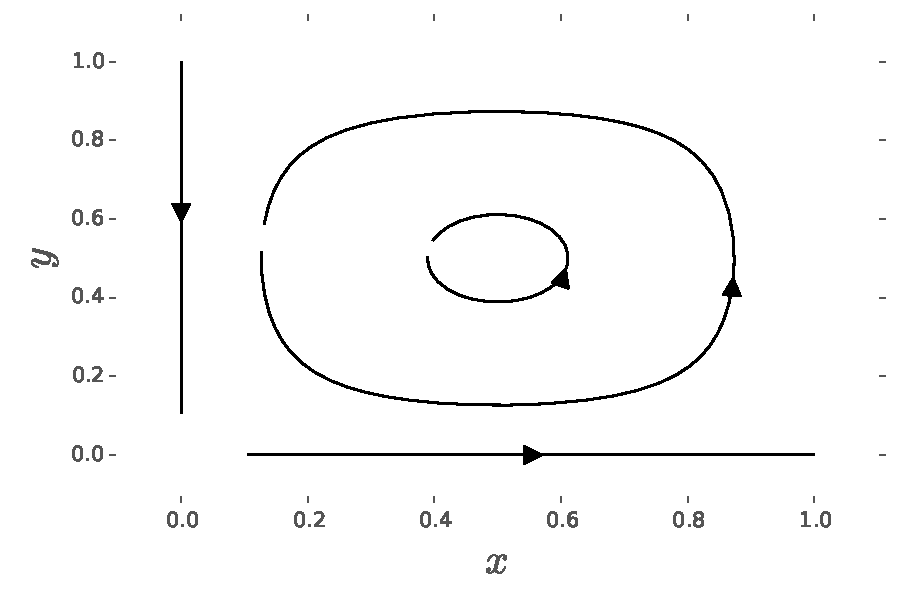
\includegraphics{skyrms-plot.pdf}
	\label{MP-phase}
	\caption{Phase diagram of replicator dynamics for matching pennies}
\end{figure}

In what follows we will largely use numerical simulations to explore the behavior of more complicated systems, but with reference to the concepts we have introduced in this section. This will allow us to explore more and more complicated systems.

%http://math.stackexchange.com/questions/761009/marginal-stability-and-centers-of-nonlinear-dynamical-systems

%http://www.theory.physics.manchester.ac.uk/~galla/lecture_notes_matching_pennies.pdf

%http://www.scholarpedia.org/article/Equilibrium#Types_of_Equilibria

\section{Signaling}
\label{Signaling}

Now that we have outlined both the static and dynamic tools used to understand behavior in games, we turn to the asymmetric sequential games of incomplete information, \emph{signaling games}, that we will use subsequently to understand both communication and language change. First, signaling games are introduced. The relevant structures and definitions are presented along with a canonical example. Second, we consider the solution concepts from the previous sections. This allows us to determine the existence and characteristics of equilibria. Finally, we consider how signaling evolves according to the replicator dynamics.

It should be noted that there are multiple traditions that have contributed to the development of signaling games. In the Economic tradition the work of \cite{harsanyi:1967,harsanyi:1968a,harsanyi:1968b} on games of incomplete information and Spence's \citeyearpar{spence:1973} model of job signaling have been central. In the Philosophical tradition, the work of \cite{lewis:1969} has been the most influential. His response to the Quinean skepticism that meaning could arise by convention has had the most direct impact on Linguistics. This account, however, rests on the assumption that speakers and hearers have perfectly-aligned interests.  This assumption will figure in the exposition of this section, mostly for the simplicity it affords us in the examples. In the next section we turn towards the consequences of loosening it.

Signaling games offer an intuitive model of communication between agents.  A signaling game consists of two players, a sender and a receiver. The sender has some private piece of information, $t \in T$, drawn according to some commonly known probability distribution, $\delta$. The piece  of information can be thought of as some fact about the state of the world. For example, we might think of it as information that the sender wants to convey to the receiver. The sender chooses a message, $m \in M$, to send to the receiver.   The receiver does not know what state of the world actually holds and must choose an action, $a \in A$, as an interpretation of the message sent. That is, the receiver is faced with the problem of inferring the state of the sender given the message.

The outcome of the game is determined by the state of the sender, the message sent, and the action taken by the receiver. The sender and the receiver have preferences over these outcomes, which are given by utility functions, $U_S$ and $U_R$ respectively, which map outcomes to real numbers: $U_S,U_R:T \times M \times A \rightarrow \mathbb{R}$. Note that the message sent can figure into the utility functions. For example, if one message is costlier than another, then the utility can be adjusted to reflect this. In what follows we will only consider costless or \emph{cheap talk} signaling where all message incur the same cost, and thus do not affect the structure of the utility functions.

As a simple example of a signaling game, consider the case where there are two states, two messages, and two actions: $T = \{t_0, t_1 \}$, $M = \{m_0, m_1 \}$, and $A = \{a_0, a_1 \}$. We can represent the structure of the game in \emph{extensive form} as in Figure \ref{SG1}. The uppermost node, labeled $\delta$, determines the likelihood of either of the two states occurring. The lines from the uppermost node represent one state or the other obtaining. The nodes labeled $S$ indicate the points in the game where the sender makes a decision regarding which message to send. The nodes labeled $R$ indicate the points where the receiver must make a decision regarding how to interpret the message. The dashed lines between receiver nodes indicates that the receiver is uncertain as to which state holds after hearing a given message. The nodes at the bottom represent the outcome and the players' preferences, as determined by the utility functions.

%{every tree node/.style={align=center,anchor=north}}
%[scale=1, level/.style={sibling distance=70mm/#1}] 

\begin{figure}[!ht]
\centering
\begin{tikzpicture}[
	scale=1, level/.style={sibling distance=70mm/#1}]
\node  (z)[circle,draw]{$\delta$}
  child {node [circle,draw] (a_left) {$S$}
    child {node  [circle,draw](left_left) {$R$}
      child {node {$1,1$}        
      edge from parent
		node[left] {$a_0$}
		node[right] {}} 
      child {node (n){$0,0$}
      edge from parent
		node[left] {}
		node[right] {$a_1$}}
    edge from parent
	node[left] {$m_0$}
	node[right] {}}
    child {node  [circle,draw](left_right) {$R$}
      child {node {$1,1$}        
      edge from parent
		node[left] {$a_0$}
		node[right] {}} 
      child {node (n){$0,0$}
      edge from parent
		node[left] {}
		node[right] {$a_1$}}
    edge from parent
	node[left] {}
	node[right] {$m_1$}}
  edge from parent
	node[left] {$t_0$ $ $}
	node[right] {}
  }
 child {node [circle,draw] (a_right) {$S$}
    child {node  [circle,draw](right_left) {$R$}
      child {node {$0,0$}        
      edge from parent
		node[left] {$a_0$}
		node[right] {}} 
      child {node (n){$1,1$}
      edge from parent
		node[left] {}
		node[right] {$a_1$}}
    edge from parent
	node[left] {$m_0$}
	node[right] {}}
    child {node  [circle,draw](right_right) {$R$}
      child {node {$0,0$}        
      edge from parent
		node[left] {$a_0$}
		node[right] {}} 
      child {node (n){$1,1$}
      edge from parent
		node[left] {}
		node[right] {$a_1$}}
    edge from parent
	node[left] {}
	node[right] {$m_1$}}
  edge from parent
	node[left] {}
	node[right] {$ $ $t_1$}
  };
\draw [dashed](left_left) to [out=35,in=-215] (right_left);
\draw [dashed](left_right) to [out=35,in=-215] (right_right);
\end{tikzpicture}
\caption{\textbf{Signaling Game:} Two states, messages, and actions. }
\label{SG1}
\end{figure}

As alluded to above, with the exception of the topmost node and the leaves, all other nodes are \emph{decision nodes}. That is, they represent those points in the game where a particular player must make a decision. An \emph{information set} consists of a set of decision nodes for a given player, which that player cannot distinguish. For example, the receiver is in an information set after hearing $m_0$. She is not sure whether she is in the node beneath state $t_0$ or $t_1$ and she must choose between $a_0$ and $a_1$. She is likewise uncertain after receiving message $m_1$. Again, her inability to distinguish the two states is indicated by a dashed line. An information set can also consist of a single decision node. For example, the sender is never uncertain about the state he is in. Thus the information sets for the sender only ever consist of a single node. 

For each player, a \emph{strategy} specifies which action to take at all \emph{information sets} for a player.\footnote{For simplicity, we only consider \emph{pure} sender (receiver) strategies, functions from states to messages (messages to actions). \emph{Mixed} strategies are a straightforward generalization. A mixed sender strategy specifies a probability distribution over pure sender strategies, $\sigma = p_1 s_1 + ... + p_k s_k$, where $\sum_i p_i = 1$. Similarly, a mixed receiver strategy specifies a probability distribution over pure receiver strategies, $\rho = q_1 r_1 + ... + q_k r_k$.} We will refer to the set of all such sender strategies as $S : [T \rightarrow M ]$, and the set of all such receiver as $R : [M \rightarrow A]$. All pure sender and receiver strategies are summarized in Figure \ref{signaling-strategies}. The sender and receiver strategies that combine to yield a one-to-one mapping from states to actions are called \emph{signaling systems}. Thus, the strategy profiles $\langle s_1, r_1 \rangle$ and $\langle s_4, r_4 \rangle$ constitute signaling systems.

\begin{figure}
\begin{center}
\begin{tikzpicture}[->,>=stealth',shorten >=1pt,auto,node distance=2cm]
  \node (A)      {$t_0$};
  \node (B) [right=2cm of A]  {$m_0$};
  \node (C) [below of=A] {$t_1$};
  \node (D) [right=2cm of C] {$m_1$};
\path[->] (A) edge node {} (B)
	  (C) edge node {} (D);
   \node (name) [below left=.5cm and .5cm of A]  {$s_1:$};
   %
     \node (D) [right=3cm of B]   {$m_0$};
  \node (E) [right=2cm of D]  {$a_0$};
  \node (F) [below of=D] {$m_1$};
  \node (G) [right=2cm of F] {$a_1$};
\path[->] (D) edge node {} (E)
	  (F) edge node {} (G);
   \node (name) [below left=.5cm and .5cm of D]  {$r_1:$};
\end{tikzpicture}
\vspace{2cm}

\begin{tikzpicture}[->,>=stealth',shorten >=1pt,auto,node distance=2cm]
  \node (A)      {$t_0$};
  \node (B) [right=2cm of A]  {$m_0$};
  \node (C) [below of=A] {$t_1$};
  \node (D) [right=2cm of C] {$m_1$};
\path[->] (A) edge node {} (B)
	  (C) edge node {} (B);
   \node (name) [below left=.5cm and .5cm of A]  {$s_2:$};
   %
     \node (D) [right=3cm of B]   {$m_0$};
  \node (E) [right=2cm of D]  {$a_0$};
  \node (F) [below of=D] {$m_1$};
  \node (G) [right=2cm of F] {$a_1$};
\path[->] (D) edge node {} (E)
	  (F) edge node {} (E);
   \node (name) [below left=.5cm and .5cm of D]  {$r_2:$};
\end{tikzpicture}\\
\vspace{2cm}

\begin{tikzpicture}[->,>=stealth',shorten >=1pt,auto,node distance=2cm]
  \node (A)      {$t_0$};
  \node (B) [right=2cm of A]  {$m_0$};
  \node (C) [below of=A] {$t_1$};
  \node (D) [right=2cm of C] {$m_1$};
\path[->] (A) edge node {} (D)
	  (C) edge node {} (D);
   \node (name) [below left=.5cm and .5cm of A]  {$s_3:$};
   %
     \node (D) [right=3cm of B]   {$m_0$};
  \node (E) [right=2cm of D]  {$a_0$};
  \node (F) [below of=D] {$m_1$};
  \node (G) [right=2cm of F] {$a_1$};
\path[->] (D) edge node {} (G)
	  (F) edge node {} (G);
   \node (name) [below left=.5cm and .5cm of D]  {$r_3:$};
\end{tikzpicture}\\
\vspace{2cm}

\begin{tikzpicture}[->,>=stealth',shorten >=1pt,auto,node distance=2cm]
  \node (A)      {$t_0$};
  \node (B) [right=2cm of A]  {$m_0$};
  \node (C) [below of=A] {$t_1$};
  \node (D) [right=2cm of C] {$m_1$};
\path[->] (A) edge node {} (D)
	  (C) edge node {} (B);
   \node (name) [below left=.5cm and .5cm of A]  {$s_4:$};
   %
     \node (D) [right=3cm of B]   {$m_0$};
  \node (E) [right=2cm of D]  {$a_0$};
  \node (F) [below of=D] {$m_1$};
  \node (G) [right=2cm of F] {$a_1$};
\path[->] (D) edge node {} (G)
	  (F) edge node {} (E);
   \node (name) [below left=.5cm and .5cm of D]  {$r_4:$};
\end{tikzpicture}\\
\vspace{2cm}


\end{center}
\caption{Sender and Receiver strategies for signaling game}
\label{signaling-strategies}
\end{figure}



The set of possible combinations of sender and receiver strategies constitute \emph{strategy profiles}. That is, a sender strategy in the set of possible sender strategies, $s \in S$, and a receiver strategy in the set of all possible receiver strategies, $r  \in R$, yield a strategy profile $\langle s,r \rangle$. Each strategy profile determines the outcome of the game. Crucially, each player's utility function depends on the state of the sender and the action taken by the receiver. That is, their respective utilities are a function of state and action. As an example, consider the case where both sender and receiver prefer successful communication. Then they both receive their preferred payoffs if there is some correspondence between the sender's state and the receiver's action. For example, in Figure \ref{SG1} both sender and receiver prefer the state and action to be the same in the following sense.

\begin{equation}
 U_{S}(t_i, a_k) = U_{R}(t_i, a_k) =
\left\{
	\begin{array}{ll}
		1  & \mbox{if } i = k \\
		0 & \mbox{else}
	\end{array}
\right.
\end{equation}
Note that this reflects the assumption that both sender and receiver have the same preference over outcomes.

Given that the different states occur with certain probabilities, and we are interested in how particular strategies do on average, we consider the expected utility for a given strategy profile. This is simply the expected value of the utility functions given the two strategies, which can be given in the case of a discrete state space as in our example above.

\begin{equation}
\begin{split}
 E[U_{S}(s,r)] &= \sum_{t} \delta (t) \cdot U_S(t, r(s(t)))\\
 E[U_{R}(s,r)] &= \sum_{t} \delta (t) \cdot U_R(t, r(s(t)))
\end{split}
\end{equation}
For each possible state the sender and receiver strategies determine an outcome. $s(t)$ is the message the sender will employ and $r(s(t))$ is the action the receiver will take given that message. The expected utility is the sum of these outcomes weighted by the probability of the state that yields them. Assuming that the two states are equiprobable, we can construct the payoff matrix for the signaling game as in Table \ref{sig-table}. Since payoffs are symmetric, only one number is presented.

\begin{table}\centering
\begin{tabular}{lllll}
\hline\noalign{\smallskip}
 & $r_1$ & $r_2$ & $r_3$ & $r_4$ \\
\noalign{\smallskip}\hline\noalign{\smallskip}
$s_1$ & $1$ & $\frac{1}{2}$  & $\frac{1}{2}$  & $0$ \\

$s_2$ & $\frac{1}{2}$ & $\frac{1}{2}$  & $\frac{1}{2}$  & $\frac{1}{2}$ \\

$s_3$ & $\frac{1}{2}$ & $\frac{1}{2}$  & $\frac{1}{2}$  & $\frac{1}{2}$ \\

$s_4$ & $0$ & $\frac{1}{2}$  & $\frac{1}{2}$  & $1$ \\

\noalign{\smallskip}\hline
\end{tabular}
\caption{Payoff matrix for signaling game}
\label{sig-table}
\end{table}
There are several Nash equilibria in the game, but only the signaling systems $\langle s_1, r_1 \rangle$ and $\langle s_4, r_4 \rangle$  are evolutionarily stable strategies, because they are the only strict Nash equilibria. In fact, given the structure of the payoffs it is possible to show that these signaling systems are the unique asymptotically stable rest points of the system, which attract the entire interior of the state space \citep[82]{hofbauer-sigmund:1998}. This means that one of the two signaling systems is almost guaranteed to evolve.


%\begin{definition}
% A strategy profile $\langle s^*, r^*\rangle$ is a \emph{Nash equilibrium}
%if and only if:
%  \begin{itemize}
%   \item For all $s \in S$, such that $s \neq s^*$, $E[U_S(s^*,r^*)] \geq
%E[U_S(s,r^*)]$
%  \item For all $r \in R$, such that $r \neq r^*$, $E[U_R(s^*,r^*)] \geq
%E[U_S(s^*,r)]$
%  \end{itemize}
%\end{definition}

%Before I prove the theorems stated in the main text, I will first prove two lemmata that will be used frequently below.
%
%Lemma 10. Let ? be a partnership game with  payoff matrix A. Then:
%
%1.	
% is evolutionarily stable if and only if  is asymptotically stable under the replicator dynamics (1) generated by A.
%2.	
%The replicator dynamics (1) for \Gamma is a Shashshahani gradient system with potential function  .
%Proof. See Hofbauer and Sigmund (1998) p.82. ?
%
%The second part of Lemma 10 implies that all solutions converge to a rest point (Akin and Hofbauer 1982). Moreover, it implies that there are no circling solutions since the average payoff V is strictly increasing along all nonstationary solutions.

\section{Behavioral dynamics}

While the simplest signaling game can be analyzed in a fairly straightforward manner, we might be interested in larger, more complicated games. For example, we might wonder about the dynamics of signaling if the state space were continuous rather than discrete. If we were to approach this by first enumerating all sender and receiver strategies, the dimensions of the system would explode exponentially. One means of controlling for this increase suggested by \cite{hofbauer-huttegger2015} is to consider behavioral strategies insofar as no information is lost in doing so (cf. \citealt{kuhn1953}).\footnote{Erol Ak\c{c}ay (p.c.) has suggested a similar approach to the problem.} The basic idea is that instead of there being a single sender population and a single receiver population, there are multiple sender and receiver populations. Each sender population corresponds to a particular state, and messages compete to be used in that state. Each receiver population corresponds to a message, and actions compete to be used in response to that message.  We start off by defining the components necessary for our analysis. Once we have defined these components we can simulate the game dynamics.


%\begin{itemize}
%	\item The relationship between mixed strategies and behavioral strategies in extensive games of perfect recall is well understood \cite{kuhn1953}. In particular, if one is interested in the equilibrium structure of extensive form games, then no essential information is lost by focusing on behavioral strategies. We propose a similar move for the evolutionary dynamics of signaling games
%%	\item The selection-mutation dynamics in behavioral strategies can be thought of as a dynamics in the entries of the sender and receiver matrices, since these matrices are nothing but a representation of the game�s behavioral strategies.
%	\item A non-injective surjective function: a surjection
%	\item Lose information, condense
%\end{itemize}



%First, we define the payoff matrices for senders and receivers, which depend solely on the utility functions of senders and receivers respectively. $\textbf{A}$ is an $n \times n$ matrix such that $\textbf{A}_{ij} = U_S(t_i, a_j)$:
%
%
%\begin{equation}
%\textbf{A} =
% \begin{pmatrix}
%  U_S(t_1, a_1) & \cdots & U_S(t_1, a_j) & \cdots & U_S(t_1, a_n) \\
%  \vdots	        & \ddots & \vdots           &           & \vdots \\
%  U_S(t_i, a_1) & \cdots & U_S(t_i, a_j) & \cdots & U_S(t_i, a_n) \\  
%  \vdots	        &  & \vdots           &   \ddots        & \vdots \\
%  U_S(t_n, a_1) & \cdots & U_S(t_n, a_j)  & \cdots & U_S(t_n, a_n) \\
% \end{pmatrix}
%\end{equation}
%$\textbf{B}$ is an $n \times n$ matrix such that $\textbf{B}_{ij} = U_R(t_i, a_j)$:
%
%\begin{equation}
%\textbf{B} =
% \begin{pmatrix}
%  U_R(t_1, a_1) & \cdots & U_R(t_1, a_j) & \cdots & U_R(t_1, a_n) \\
%  \vdots	        & \ddots & \vdots           &           & \vdots \\
%  U_R(t_i, a_1) & \cdots & U_R(t_i, a_j) & \cdots & U_R(t_i, a_n) \\  
%  \vdots	        &  & \vdots           &   \ddots        & \vdots \\
%  U_R(t_n, a_1) & \cdots & U_R(t_n, a_j)  & \cdots & U_R(t_n, a_n) \\
% \end{pmatrix}
%\end{equation}
%
%
%Second, we define the sender and receiver populations. $\textbf{X}$ is a stochastic population matrix such that the proportion of the population in $x_i$ using $m_j$ is $x_{ij}$, with $\sum_j x_{ij} = 1$.
%
%\begin{equation}
%\textbf{X} =
% \begin{pmatrix}
%  x_{11} &  x_{12} & x_{13} \\
%  \vdots        & \vdots & \vdots \\
%  x_{i1} &  x_{i2} & x_{i3} \\
%  \vdots	& \vdots    & \vdots \\
%  x_{n1} &  x_{n2} & x_{n3} \\
% \end{pmatrix}
%\end{equation}
% 
%Intuitively, each row corresponds to a given state. Each element in the row corresponds to the proportion of use in that population.  Each row sums to one because the proportion using the various  signals must sum to one.
% 
%$\textbf{Y}$ is a population matrix such that the proportion of the population in $y_i$ responding with action $a_j$ is $y_{ij}$, with $\sum_j y_{ij} = 1$.
%
%\begin{equation}
%\textbf{Y} =
% \begin{pmatrix}
%  y_{11} & \cdots & y_{1j}  & \cdots & y_{1n} \\
%  y_{21} & \cdots & y_{2j}  & \cdots & y_{2n} \\
%  y_{31} & \cdots & y_{3j}  & \cdots & y_{3n} \\
% \end{pmatrix}
%\end{equation}
%
%Again, intuitively, each row corresponds to a given message. Each element in the row corresponds to the proportion of different responses to the message. Each row sums to one because the proportion using the various responses must sum to one.
% 
% 
%The expected utility of sending message $m_j$ in state $t_i$, where $\textbf{Y}^T$ is the transpose of $\textbf{Y}$:
%
%\begin{equation}
%	E [ x_{ij} ] = (\textbf{A}\textbf{Y}^T)_{ij}
%\end{equation}
%
%The average expected utility in a sender population $x_i$:
%
%\begin{equation}
%	E [ x_{i} ] = (\textbf{X}(\textbf{A}\textbf{Y}^T)^T)_{ii}
%\end{equation}
%
%This gives the replicator dynamic for a given message in a sender population.
%\begin{equation}
%	\dot{x}_{ij} = x_{ij}((\textbf{A}\textbf{Y}^T)_{ij} - (\textbf{X}(\textbf{A}\textbf{Y}^T)^T)_{ii})
%\end{equation}
%
%
%
%
%$\textbf{P}$ is a stochastic matrix such that $\forall i \textbf{P}_i = P(t_1),...,P(t_n)$. That is, $\textbf{P}$ is just $n$ rows of the prior probability distribution over states.
%
%\begin{equation}
%\textbf{P} =
% \begin{pmatrix}
%  P(t_1) & \cdots & P(t_i)  & \cdots & P(t_n) \\
%  \vdots &  & \vdots  & & \vdots  \\
%  P(t_1) & \cdots & P(t_i)  & \cdots & P(t_n) \\
% \end{pmatrix}
%\end{equation}
%
%
%Now that we have defined the  replicator dynamics for the sender populations, we can do the same for the receiver populations with a few additions. Let $\textbf{C}$ be the conditional probability of a state given a message. That is, $\textbf{C}_{ij} = P(t_i | m_j)$, where $\otimes$ indicates element-wise Hadamard multiplication and $\oslash$ indicates the element-wise Hadamard division.
%
%\begin{equation}
%\textbf{C} = (P^T \otimes X) \oslash (PX)
%\end{equation}
%
%
%The expected utility of receiver responding to message $m_i$ with action $a_j$:
% 
%\begin{equation}
%	E [ y_{ij} ] = (\textbf{B}^T\textbf{C})_{ji}
%\end{equation}
%
%Since the resulting matrix is $n \times m$, we swap the indices to get the appropriate value. Each column corresponds to a receiver population, and each row corresponds to a response action.
%
%The average expected utility in a receiver population $y_i$:
%
%\begin{equation}
%	E [ y_{i} ] = (Y(\textbf{B}^T\textbf{C})_{ji})_{ii}
%\end{equation}
%
%The replicator dynamic for a given action in response to a message is given by the following.
%
%\begin{equation}
%		\dot{y}_{ij} = y_{ij}(\textbf{B}^T\textbf{C})_{ji} - (Y(\textbf{B}^T\textbf{C})_{ji})_{ii})
%\end{equation}
%Together these behavioral replicator dynamics can be used to investigate any signaling game with a finite number of states, messages, and actions.

\subsection{The Simplest Signaling Game}

To begin, we apply this new framework to the simplest non-trivial signaling game where we have two equiprobable states, two messages, and two actions. The structure of the behavioral  replicator dynamics is determined by the structure in Figure \ref{behavioral-dynamics}. $x_0$ represents the probability that $m_0$ will be used in the $t_0$ sender population. Likewise $x_1$ represents the probability that $m_1$ will be used in the $t_1$ sender population. The dotted lines indicates probabilities that can be derived from others. All told, then, the behavioral replicator dynamic  for this signaling game gives rise to a four-dimensional system.

\begin{figure}
\begin{center}
\begin{tikzpicture}[->,>=stealth',shorten >=1pt,auto,node distance=3cm]
  \node (A)      {$t_0$};
  \node (B) [right of=A]  {$m_0$};
  \node (C) [right of=B] {$a_0$};
  \node (D) [below of=A] {$t_1$};
  \node (E) [right of=D] {$m_1$};
  \node (F) [right of=E] {$a_1$};
\path[->] (A) edge node {$x_0$} (B)
	  (A) edge[dashed,pos=0.85] node {} (E)
	  (B) edge node {$y_0$} (C)
	  (B) edge[dashed,pos=0.85] node {} (F)
	  (D) edge[below] node {$x_1$} (E)
	  (D) edge[dashed,pos=0.75] node {} (B)
	  (E) edge[below] node {$y_1$} (F)
	  (E) edge[dashed,pos=0.75] node {} (C);
\end{tikzpicture}
\end{center}
\caption{Signaling game in behavioral space}
\label{behavioral-dynamics}
\end{figure}

We will generalize the parameters a bit to match the simpler games we used above. Namely, let the sender and receiver payoffs be the following matrices, with parameters $\alpha$ and $\beta$.

\begin{equation}
\mathbf{A} =
 \begin{pmatrix}
  1 - \alpha & \alpha \\
  \beta & 1 - \beta \\
 \end{pmatrix}
\end{equation}

\begin{equation}
\mathbf{B} =
 \begin{pmatrix}
  1 & 0 \\
  0 & 1 \\
 \end{pmatrix}
\end{equation}
These yield the general behavioral sender and receiver replicator dynamics.

\begin{equation}
	\begin{split}
		\dot{x}_0 &= x_0(1-x_0)(y_0 + y_1 - 1)(1 - 2\alpha)\\	
		\dot{x}_1 &= x_1(1-x_1)(y_0 + y_1 - 1)(1 - 2\beta)\\
	\end{split}
\end{equation}

\begin{equation}
	\begin{split}
		\dot{y}_0 &= y_0(1 - y_0)\left(\frac{x_0 + x_1 - 1}{x_0 - x_1 + 1}\right)\\
		\dot{y}_1 &= y_1(1 - y_1)\left(\frac{x_0 + x_1 - 1}{x_1 - x_0 + 1} \right)\\
	\end{split}
\end{equation}

 The case where $\alpha = \beta = 0$ corresponds to the lewis signaling game we introduced in the previous section, which is also related to the coordination game we started with. This is a signaling games with common interests. The case where $\alpha = \beta = 1$ corresponds to signaling with matching pennies. This is a signaling game with conflicting interests.  The cases where $\alpha = 0, \beta = 1$  and $\alpha = 1, \beta = 0$ also offer an interesting comparison. These are games of at least partial common interest. We address each of these below.

\subsection{Common Interests}

Since the receiver dynamics do not vary as we change the parameters, we omit them. Under common interests the sender dynamics are the following.

\begin{equation}
	\begin{split}
		\dot{x}_0 &= x_0(1-x_0)(y_0 + y_1 - 1)\\	
		\dot{x}_1 &= x_1(1-x_1)(y_0 + y_1 - 1)\\
	\end{split}
\end{equation}

Typical results for a numerical solution are shown in Figure \ref{common-interests}, where we plot $x_0$ against $y_0$ and $x_1$ against $y_1$, with circles represent the starting state of both of trajectories. That is, we represent the four-dimensional system as two two-dimensional systems overlaid on each other. The established result is exactly what we see. Namely, the system either converges to the origin or to the upper right-hand corner. Referring back to Figure \ref{behavioral-dynamics} it is clear that these constitute the signaling systems of the signaling game as we described them. That is, these are the points that guarantee a one-to-one mapping between states and actions.


\begin{figure}
	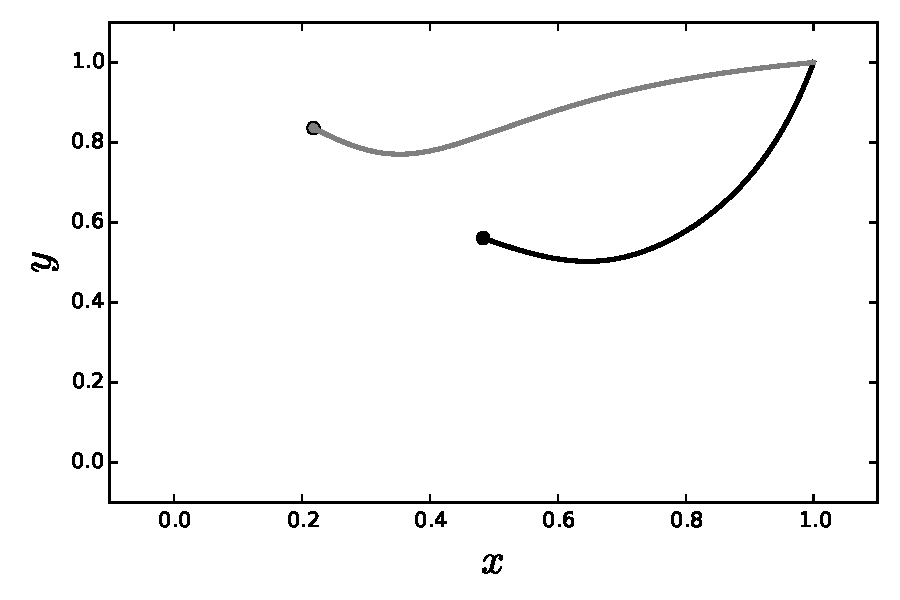
\includegraphics{common-interests.pdf}
	\label{common-interests}
	\caption{Solution trajectories for behavioral replicator dynamics for common interest signaling}
\end{figure}


%\begin{equation}
%	\mathbf{J} 
%	 =
%	 \begin{bmatrix} 
%	(- 2 x_{0} + 1) (y_{0} + y_{1} - 1) & 0 & x_{0} (- x_{0} + 1) & x_{0} (- x_{0} + 1)\\
%	0 & (- 2 x_{1} + 1) (y_{0} + y_{1} - 1) & x_{1} (- x_{1} + 1) & x_{1} (- x_{1} + 1)\\
%	\frac{2 y_{0} (x_{1} - 1) (y_{0} - 1)}{(x_{0} - x_{1} + 1)^{2}} & - \frac{2 x_{0} y_{0} (y_{0} - 1)}{(x_{0} - x_{1} + 1)^{2}} & \frac{(- 2 y_{0} + 1) (x_{0} + x_{1} - 1)}{x_{0} - x_{1} + 1} & 0 \\
%	- \frac{2 x_{1} y_{1} (y_{1} - 1)}{(- x_{0} + x_{1} + 1)^{2}} & \frac{2 y_{1} (x_{0} - 1) (y_{1} - 1)}{(- x_{0} + x_{1} + 1)^{2}} & 0 & \frac{(- 2 y_{1} + 1) (x_{0} + x_{1} - 1)}{- x_{0} + x_{1} + 1}\\
%	 \end{bmatrix}
%\end{equation}
%
%It's clear that both $\frac{\partial \dot{y}_0}{\partial x_0}$ and $\frac{\partial \dot{y}_1}{\partial x_0}$ go to infinity as we approach points at the edge of the state space.

%\begin{figure}
%	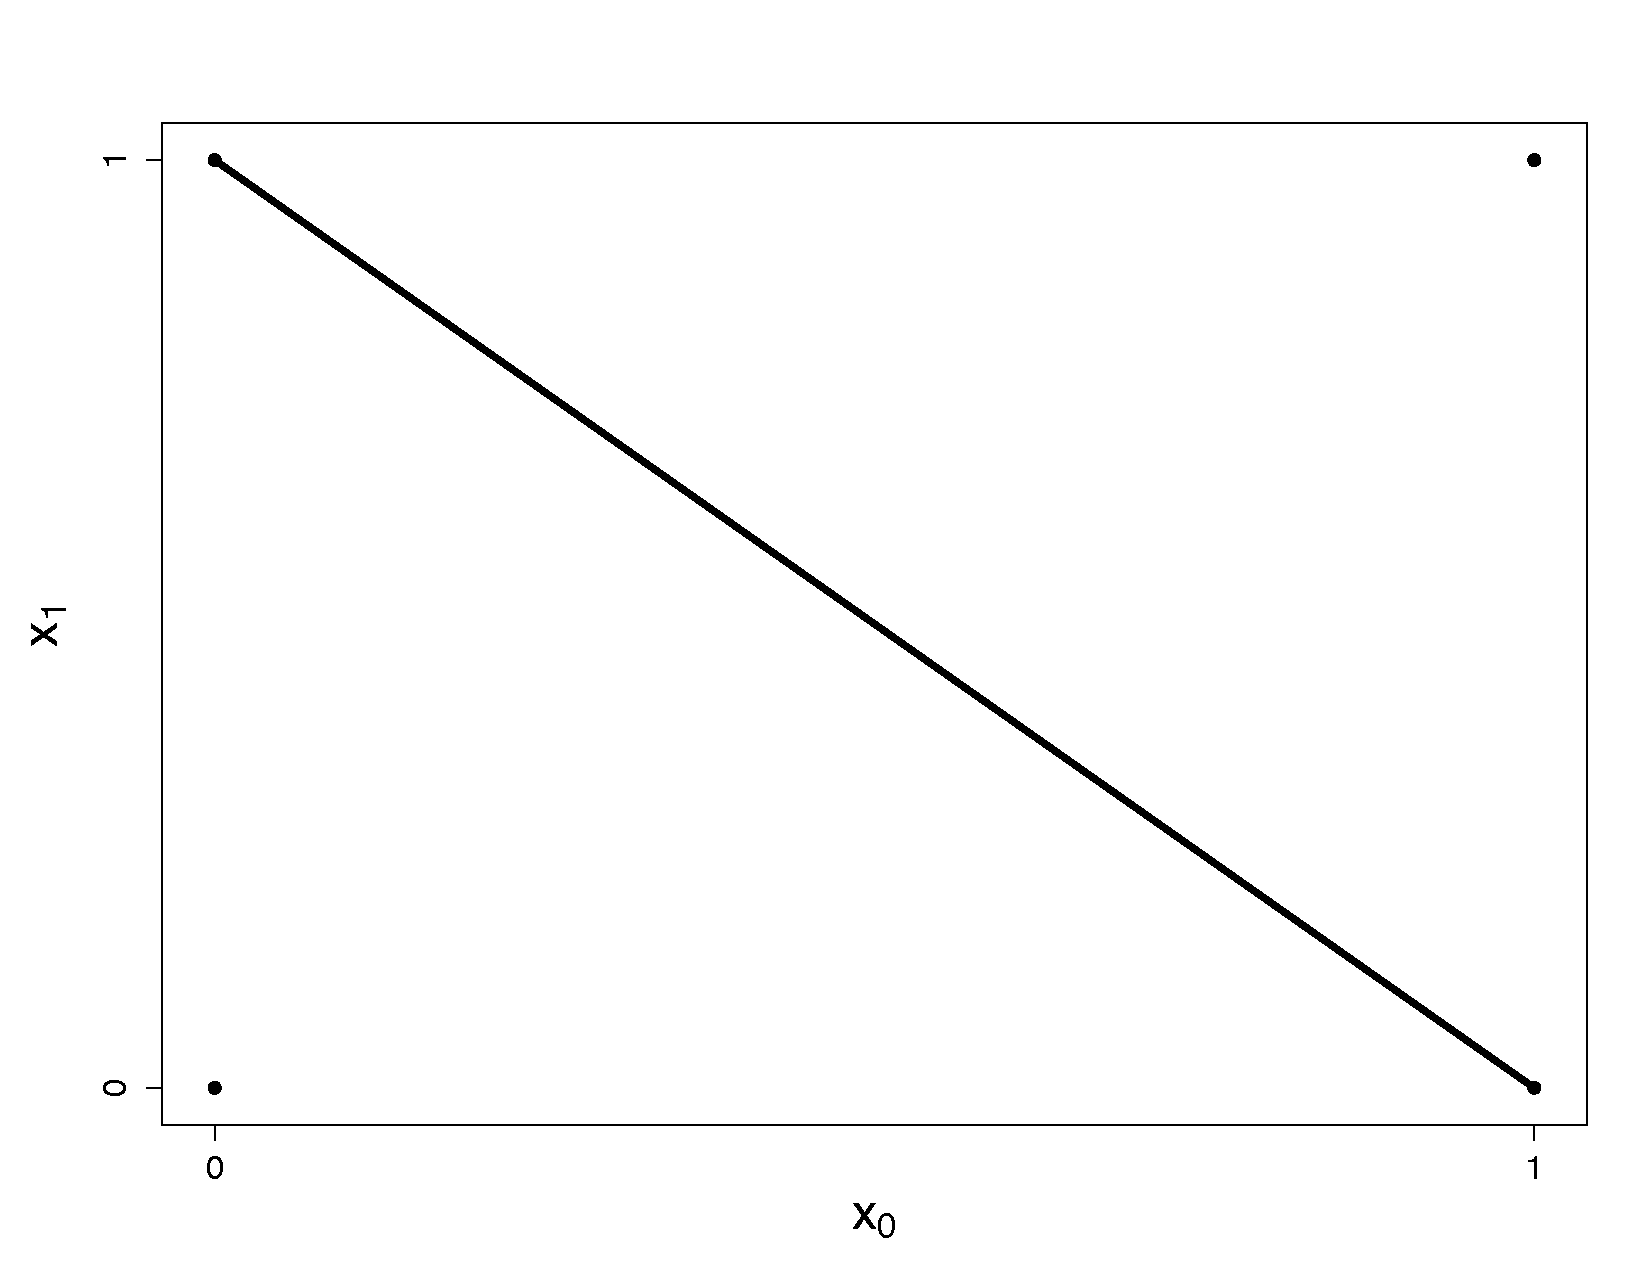
\includegraphics[width=.5\textwidth]{lewis-phase-portrait-senders}	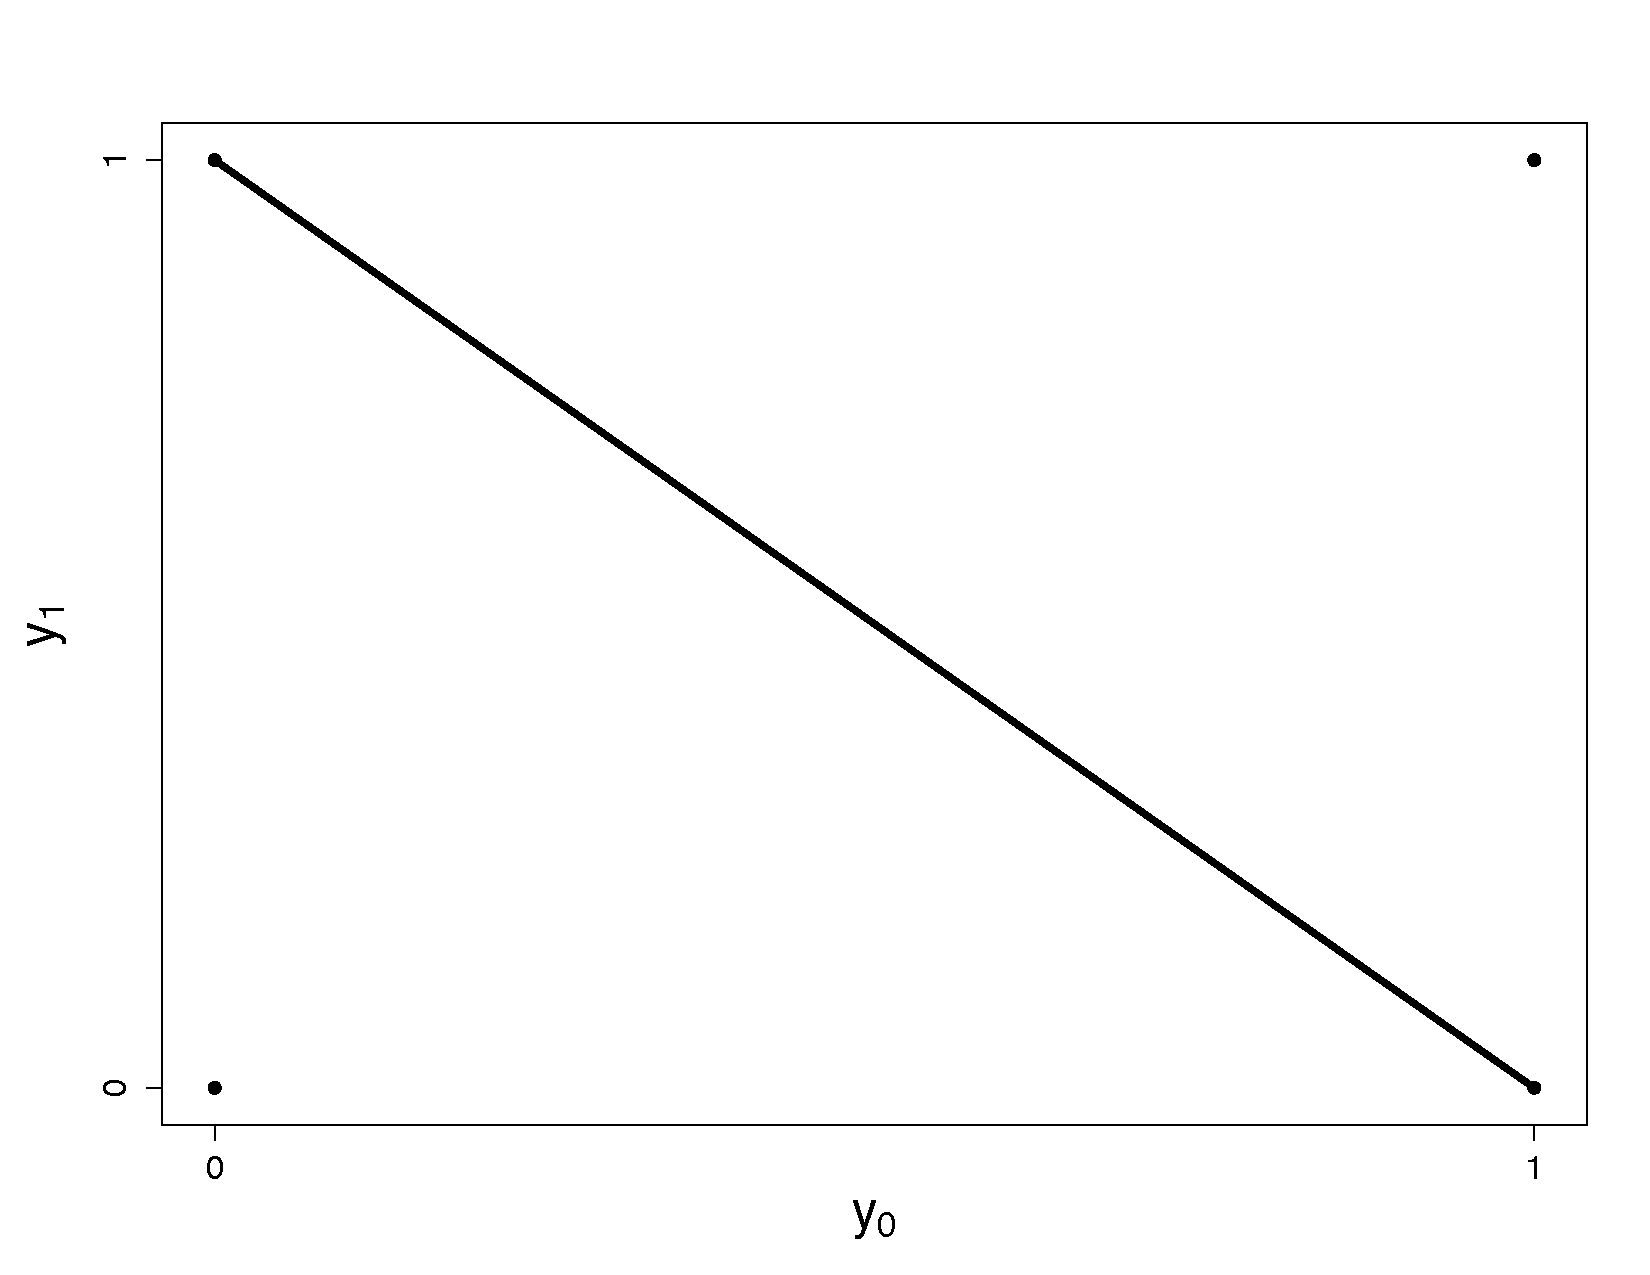
\includegraphics[width=.5\textwidth]{lewis-phase-portrait-receivers}		
%\end{figure}


\subsection{Conflicting Interests}

If we alter the payoff structure to reflect that of matching pennies, then the following behavioral sender dynamics result.
\begin{equation}
	\begin{split}
		\dot{x}_0 &= x_0(1-x_0)(1 - y_0 - y_1)\\	
		\dot{x}_1 &= x_1(1-x_1)(1 - y_0 - y_1)\\
	\end{split}
\end{equation}

Typical results for numerical solution are shown in Figure \ref{conflicting-interests}. Interestingly, much like in the case of matching pennies, the system exhibits closed orbits.

\begin{figure}
	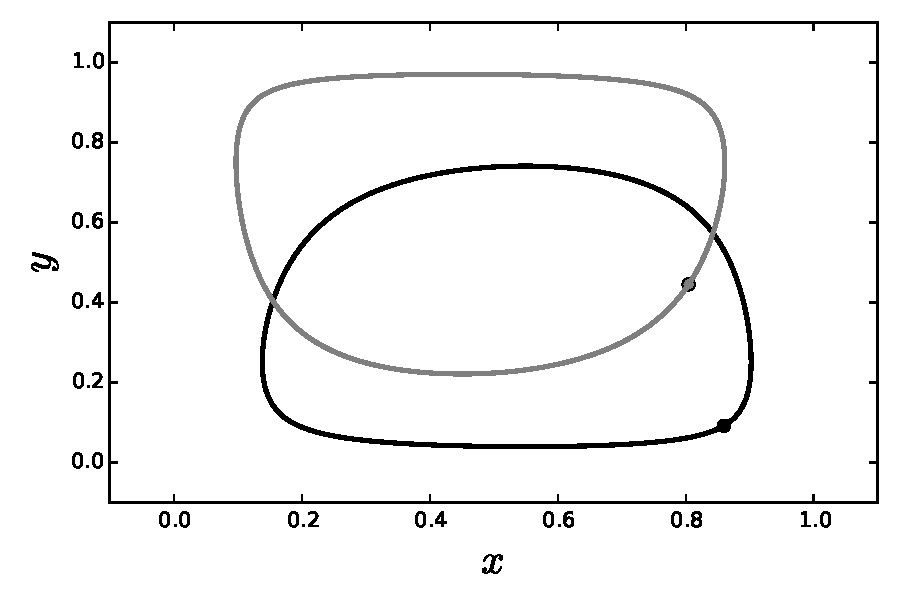
\includegraphics{conflicting-interests.pdf}
	\label{conflicting-interests}
	\caption{Solution trajectories for behavioral replicator dynamics for conflicting interest signaling}
\end{figure}

An interesting consequence of this behavior is that despite the fact that the sender does not want to signal what action he is going to take, there is some amount of information carried by the signal. This can quantified by calculating the \emph{Kullback-Leibler divergence} or \emph{information gain} due to the signal.

\begin{equation}
	KL(m) = \sum_t P(t \mid m) log \left( \frac{P(t \mid m)}{P(t)} \right)
\end{equation}
The basic intuition behind this formula is that it allows us a way to compare the receiver's expectations prior to receiving the message, which is determined by the probability distribution over states, to the posterior distribution after having heard the message.  The difference between these two distributions is the information gained by having received the message. The average information gain for the two signals is shown in Figure \ref{conflicting-interests-KL}. As a point of reference, if the messages perfectly corresponded to states, as they do in a signaling system, then the average information gain would be equal to one. In other terms, the information gained from the signal would be one bit, because it would allow us to distinguish between two equiprobable states.s

\begin{figure}
	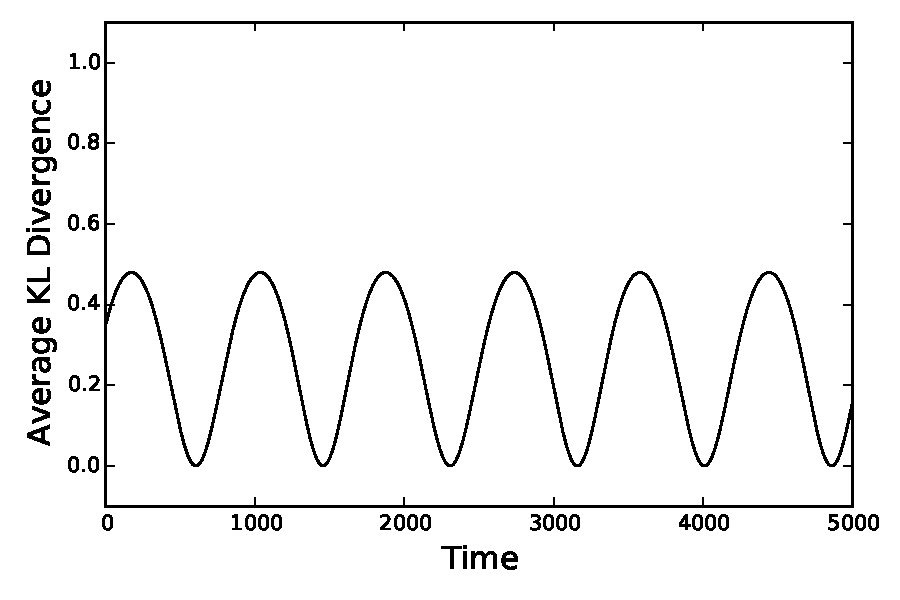
\includegraphics{conflicting-interests-KL.pdf}
	\label{conflicting-interests-KL}
	\caption{Average Kullback-Leibler Divergence for signals under conflicting interests}
\end{figure}

The fact that signals still carry information, even under diametrically opposed interests is both interesting and surprising (cf. \citealt{sato-etal2002,wagner2012}).

%\subsection{Partial Common Interests}
%
%Perhaps even more surprising is the case of only partially misaligned interests, or as \cite{blume-etal:2001} refer to them, \emph{partial common interests}. That is, when $\alpha = 0, \beta = 1$  and $\alpha = 1, \beta = 0$, then at least some of the time senders want to accurately signal their type. Consider the case where $\alpha = 1, \beta = 0$, which yields the following behavioral dynamics.
%
%\begin{equation}
%	\begin{split}
%		\dot{x}_0 &= x_0(1-x_0)(1 - y_0 - y_1)\\	
%		\dot{x}_1 &= x_1(1-x_1)(y_0 + y_1 - 1)\\
%	\end{split}
%\end{equation}
%
%\begin{figure}
%	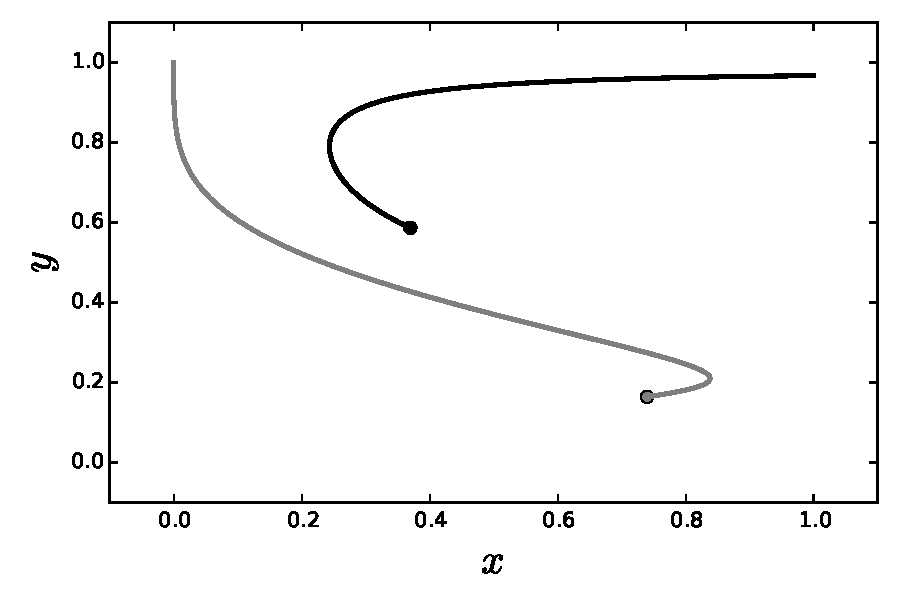
\includegraphics{partial-common-interests.pdf}
%	\label{partial-common-interests}
%	\caption{Solution trajectories for behavioral replicator dynamics for partial common interest signaling}
%\end{figure}
%
%Typical results for a numerical solution are presented in Figure \ref{partial-common-interests}. The sender populations converge to opposite sides of the state space, meaning that senders all converge on using the same signal. In response to this, receivers converge to some intermediate response, although not necessarily the one that might be expected from the distribution over states. The most striking thing about this case is that it differs dramatically from the case where interests are perfectly opposed. In the first case no information is carried by the messages, whereas there is always some information carried by messages in the second.


\section*{Summary}

In this chapter we outlined the basic framework that will be used subsequently. We noted the complementary role of static and dynamic methods for understanding the evolution of populations. We also presented a general method for describing the dynamics of signaling games and noted interesting properties of the simplest kind of signaling game. We now turn to our application of this framework to the functional Jespersen cycle.
